\documentclass{article}
\usepackage[utf8]{inputenc}
\usepackage{geometry}
\usepackage{fullpage}
\usepackage{ctex}
\usepackage{float}
\usepackage{graphicx}
\usepackage{subfigure}
\usepackage{hyperref, wrapfig,fancybox,listings,subfigure}

\lstset{numbers=left,
keywordstyle=\color{blue!70}, commentstyle=\color{red!50!green!50!blue!50},
frame=shadowbox,
rulesepcolor=\color{red!20!green!20!blue!20},
breaklines=true,
extendedchars=true
}

\title{Colorization using Optimization}
\author{王世因 2016011246}
\date{}
\begin{document}
\maketitle

\tableofcontents
\newpage

\section{算法简介}
在YIQ和YUV图片格式中,Y代表图片的亮度,含有各种阴影细节,单独输出后就可以得到黑白照片。我在算法实现中使用的是YIQ格式,是美洲和日韩电视机使用的格式。算法假设距离近的点中,灰度Y差距小的点,它们的色彩差距也会小。因此我们可以将这个问题转化成一个最小化$J(I)$和$J(Q)$的优化问题。
\begin{equation}
w_{rs} \propto e^{-\frac{(Y(r)-Y(s))^2}{2\sigma_r^2}}
\end{equation}


\begin{equation}
J(I) = \sum_r (I(r)-\sum_{s\in N(r)} w_{rs} I(s))^2
\end{equation}

\begin{equation}
J(Q) = \sum_r (Q(r)-\sum_{s\in N(r)} w_{rs} Q(s))^2
\end{equation}

在艺术家着色的草图中,部分点的色彩是给定的:如果是白色就是说明要保留原图的色彩,如果是其他颜色就是把这部分色彩变成新上的颜色。把白色的点的集合记为$White$,把其他颜色的点的集合记为$Color$。把一个像素相邻的点记为$N(i, j)$

最小值在$J'(I)=0$和$J'(Q)=0$时取到,也就是解下面的方程:

\begin{equation}
W_{i, j} = \left\{
\begin{array}{cc}
1 & i=j\\
-w_{ij} & i\neq j, i\in N(j), i\notin White \cap Color\\
0 & otherwise
\end{array}
\right.
\end{equation}

\begin{equation}
b_i= \left\{
\begin{array}{cc}
sketch(i) & i\in Color\\
origin(i) & i\in White\\
0 & otherwise
\end{array}
\right.
\end{equation}

\begin{equation}
WI = b_1
\end{equation}


\begin{equation}
WQ = b_2
\end{equation}

注意到因为W矩阵只在两个点相邻的情况下才可能取非零的值,每个点的相邻点很少,所以它是一个稀疏的矩阵,我使用了scipy中的csc格式来存储和求解,提升计算效率。

因为我的笔记本的计算资源有限,我事先对图片进行了$2\times 2$的压缩,最后把输出再进行差值,提升了运算效率。


\section{图像处理}
在frame.py中,StaticFrame代表了静态图片的处理,执行脚本是color.py。使用的方法为:

\begin{lstlisting}[language=bash]
 python3 color.py images/gray_0.png images/sketch_0.png images/result_0.png images/weights/0.pickle
\end{lstlisting}

依次输入原始图片位置、上色草图位置、输出图片位置和预存的权重的位置(如果事先没有权重的话就是计算好的权重应该存储的位置)。

\subsection{图像着色结果}


\begin{figure}[H]
\centering
\subfigure{
\begin{minipage}[t]{0.3\linewidth}
\centering
\includegraphics[width=\linewidth]{gray_0.png}
\caption{gray}
\end{minipage}%
}%
\subfigure{
\begin{minipage}[t]{0.3\linewidth}
\centering
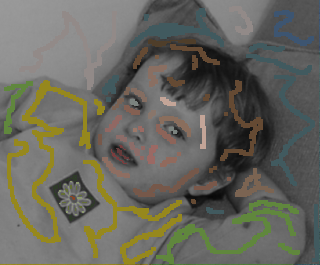
\includegraphics[width=\linewidth]{sketch_0.png}
\caption{sketch}
\end{minipage}%
}%
\subfigure{
\begin{minipage}[t]{0.3\linewidth}
\centering
\includegraphics[width=\linewidth]{result_0.png}
\caption{result}
\end{minipage}
}%
\centering
\end{figure}



\begin{figure}[H]
\centering
\subfigure{
\begin{minipage}[t]{0.3\linewidth}
\centering
\includegraphics[width=\linewidth]{gray_5.png}
\caption{gray}
\end{minipage}%
}%
\subfigure{
\begin{minipage}[t]{0.3\linewidth}
\centering
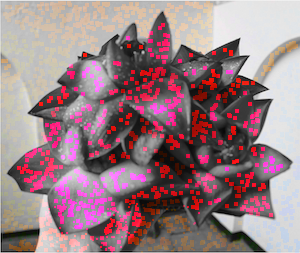
\includegraphics[width=\linewidth]{sketch_5.png}
\caption{sketch}
\end{minipage}%
}%
\subfigure{
\begin{minipage}[t]{0.3\linewidth}
\centering
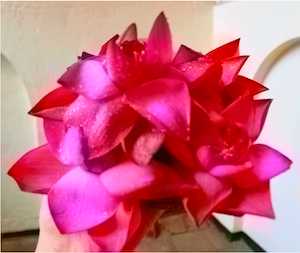
\includegraphics[width=\linewidth]{result_5.png}
\caption{result}
\end{minipage}
}%
\centering
\end{figure}

\subsection{图像换色结果}

\begin{figure}[H]
\centering
\subfigure{
\begin{minipage}[t]{0.3\linewidth}
\centering
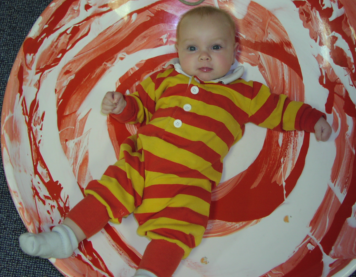
\includegraphics[width=\linewidth]{gray_21.png}
\caption{origin}
\end{minipage}%
}%
\subfigure{
\begin{minipage}[t]{0.3\linewidth}
\centering
\includegraphics[width=\linewidth]{sketch_21.png}
\caption{sketch}
\end{minipage}%
}%
\subfigure{
\begin{minipage}[t]{0.3\linewidth}
\centering
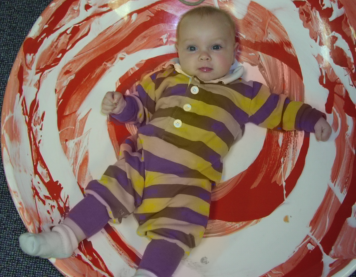
\includegraphics[width=\linewidth]{result_21.png}
\caption{result}
\end{minipage}
}%
\centering
\end{figure}



\begin{figure}[H]
\centering
\subfigure{
\begin{minipage}[t]{0.3\linewidth}
\centering
\includegraphics[width=\linewidth]{gray_13.png}
\caption{origin}
\end{minipage}%
}%
\subfigure{
\begin{minipage}[t]{0.3\linewidth}
\centering
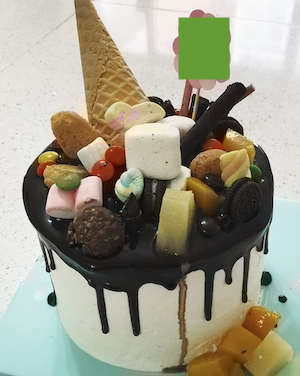
\includegraphics[width=\linewidth]{sketch_13.png}
\caption{sketch}
\end{minipage}%
}%
\subfigure{
\begin{minipage}[t]{0.3\linewidth}
\centering
\includegraphics[width=\linewidth]{result_13.png}
\caption{result}
\end{minipage}
}%
\centering
\end{figure}

\section{从静态图片扩展到视频}
我首先使用cv2.VideoCapture把视频分成若干帧的形式。在路径下使用“gray”文件夹来存储所有的原始视频的帧(黑白帧或者是着色前的图片),使用“sketch”来存储艺术家上色的草图帧。然后在命令行中执行命令:

\begin{lstlisting}[language=bash]
 python3 video_dynamic.py videos/butterfly
\end{lstlisting}

\subsection{准静态图片的像素采样法}
这部分算法对应代码文件$video\_color.py$,我通过在上一帧图片中获得一些采样点来,作为本帧的标注色彩。因为我采用的是30帧一秒的视频质量,视频中相邻两帧间的变化不大,所以可以直接进行一定的色彩继承分析。因为优化算法最小化的是总体的灰度匹配概率,因为部位微小位移造成的标注误差可以在最优化求解的时候被补偿。相比下面的这种方法,本方法因为没有增加权重矩阵的大小,所以计算起来更快,占用的计算资源也更小。

\begin{figure}[H]
\centering
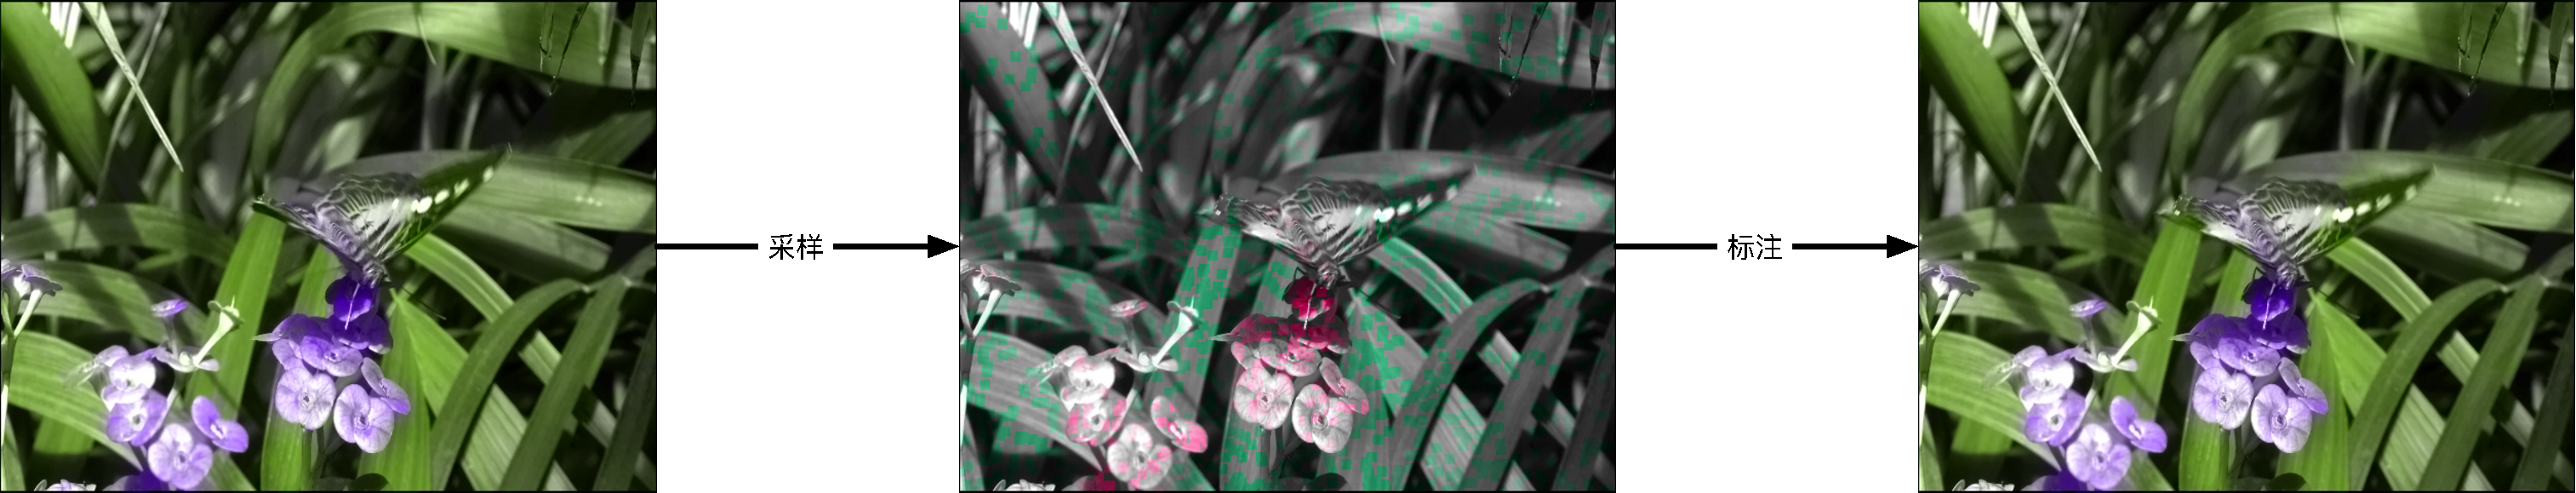
\includegraphics[scale=0.3]{seq.pdf}
\caption{相邻帧之间采样标注色彩}
\end{figure}

\subsection{位移捕捉和临点检测}
这是原文中提到的方法,通过算法Lucas-Kanade计算各个像素点的运动情况,找到相邻两帧中对应的点,拓展静态图片中像素点的临点,再进行求解。
\begin{equation}
Y_t(p) +  \nabla Y_{(x, y)} v = 0
\end{equation}

\begin{equation}
\left[
\begin{array}{cc}
Y_x(p_1) & Y_y(p_1)\\
Y_x(p_2) & Y_y(p_2)\\
Y_x(p_3) & Y_y(p_3)\\
\ldots & \ldots \\
Y_x(p_{25}) & Y_y(p_{25})\\
\end{array}
\right]
\left[
\begin{array}{c}
v_x\\
v_y
\end{array}
\right]
= - 
\left[
\begin{array}{c}
Y_t(p_1)\\
Y_t(p_2)\\
Y_t(p_3)\\
\ldots\\
Y_t(p_{25})\\
\end{array}
\right]
\end{equation}

\begin{equation}
||(x_{t+1}-v_x, y_{t+1}-v_y) - (x_t, v_t)||< T
\end{equation}

在具体的实现上,我根据上面的公式生成一个包含两帧的权重矩阵,重新跑一边静态图片的上色算法,得到后一帧的色彩。因为权重矩阵是一个很大的稀疏矩阵,这个做法的权重矩阵是静态图片权重矩阵的四倍,显著地增加了耗时。对比来看,这个方法适用于移动迅速的图片和每秒帧数少的图片。相应的代码实现在$video\_dynamic.py$中,对应$frame.DynamicFrame$类。

\section{算法的不足}

\paragraph{算法假设}算法假设蕴含的逻辑是,一个色彩相同区域的灰度是基本上一样的,而且不同色块间的灰度有一定的大小差距。然而,在一些表面纹理复杂的物体中,同一个色块的灰度变化挺大;在漫画或者过度曝光的照片中,不同的色块中并没有很多的灰度差距。比如下面的这个画面来自1928年的电影《威力号汽船》,会出现大片的白色,缺少灰度的变化,而且白色的内部的灰度的变化没有什么规律。
\begin{figure}[H]
\centering
\includegraphics[scale=2]{gray_9.jpeg}
\caption{《威力的汽船》剧照}
\end{figure}

\paragraph{工作量}本方法需要艺术家进行人为的色彩标注,对于处理长视频来说是一个任务量很大的工作。而且随着图片精度的提高,权重矩阵的大小也迅速增长,计算的时间变得很长,影响效率。


\paragraph{}


\end{document}